
\chapter{HPC Software Stack}

\begin{figure}[H]
    \centering
    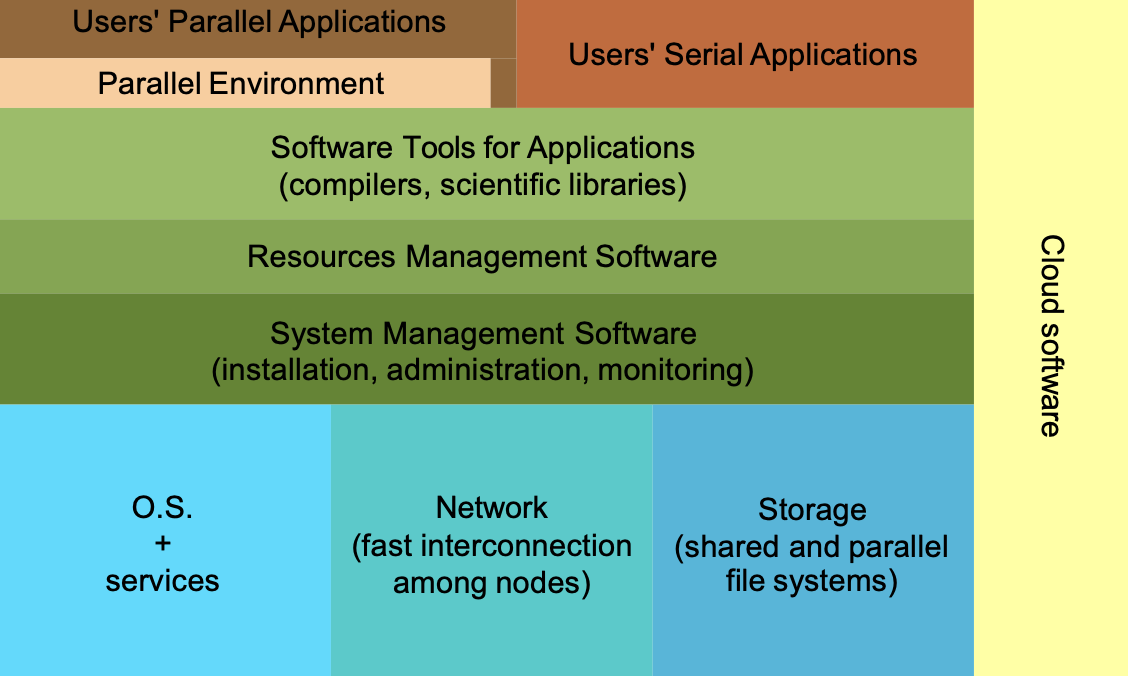
\includegraphics[width=0.8\textwidth]{assets/fig13.png}
    \caption{What we need}
    \label{fig:hpc_software_stack}
\end{figure}

We refer to \textbf{Cluster Middleware} as the software stack that is used to manage the cluster. It is composed of several layers, each one with its own purpose. The first layer is the \textbf{Operating System}, which is the base layer of the stack. The second layer is the \textbf{Resource Manager}, which is used to manage the resources of the cluster. The third layer is the \textbf{Job Scheduler}, which is used to schedule the jobs on the cluster.

\begin{itemize}
    \item The \textbf{Administration Software} is used to manage the cluster. It is used to install, configure, and monitor the cluster. It is also used to manage the users and groups on the cluster.
    \item The \textbf{Resource management and scheduling software (LRMS)} takes care of having many users and distribute process, balances the load among different users and schedules multiple tasks.
\end{itemize}

\section{Resource Management Problem}

Once we have a pool of users and a pool of resources, then some software is needed to control the available resources, to decide which application to execute based on available resources and to execute applications.

\begin{figure}[H]
    \centering
    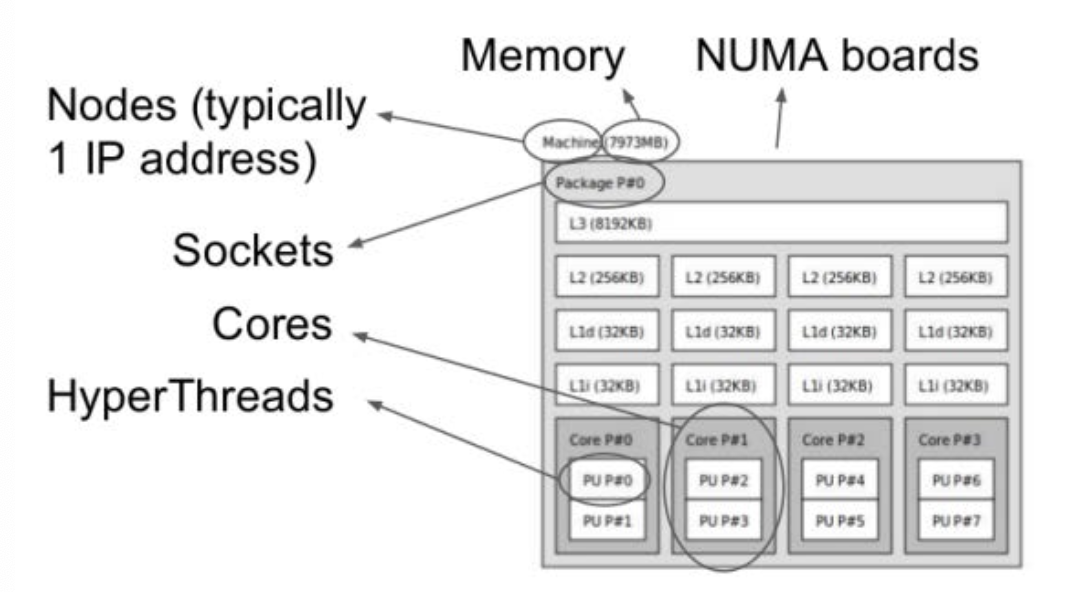
\includegraphics[width=0.8\textwidth]{assets/fig14.png}
    \caption{HPC resources}
    \label{fig:hpc_resources}
\end{figure}

plus:
\begin{itemize}
    \item network resources 
    \item GPU/Accelerator 
    \item Software resources 
\end{itemize}

Let's now define some terms:
\begin{itemize}
    \item \textbf{Batch Scheduler}: a software that manages the execution of jobs in a batch mode. It is used to schedule the jobs on the cluster.
    \begin{observationblock}[Scheduling]
        \plaintt{Scheduling} is the process of assigning resources to jobs.
    \end{observationblock}
    \begin{figure}[H]
        \centering
        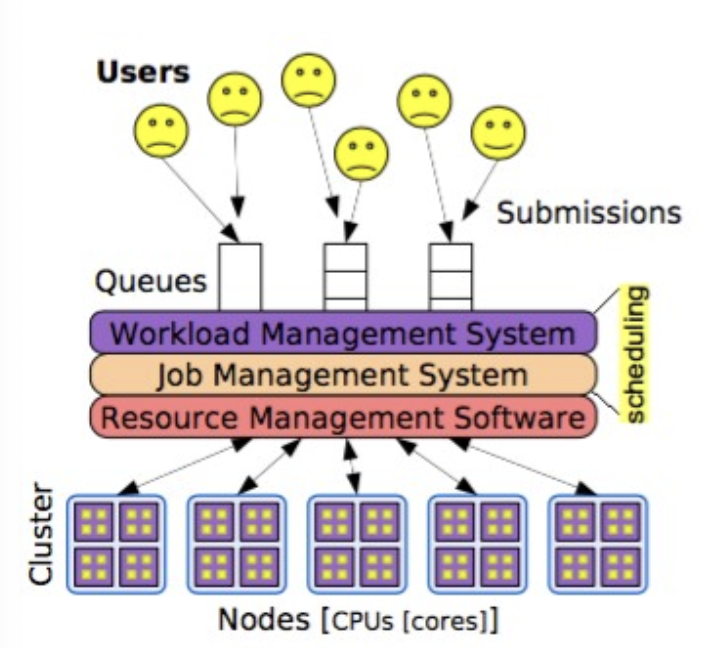
\includegraphics[width=0.5\textwidth]{assets/fig15.png}
        \caption{Batch scheduler}
        \label{fig:scheduling}
    \end{figure}
    \item \textbf{Resources Manager}: software that enable the jobs to connect the nodes and run. 
    \item \textbf{Node (aka Computing Node)}: computer used for its computational power.
    \item \textbf{Login/Master node}: it's through this node that the users will submit/launch/manage jobs.
\end{itemize}


\begin{definitionblock}[SLURM]
    SLURM (Simple Linux Utility for Resource Management) is an open-source job scheduler for Linux and Unix-like kernels, used by many of the world's supercomputers and computer clusters.
\end{definitionblock}

\begin{itemize}
    \item \textbf{Jobs}: Resource allocation requests.
    \item \textbf{Job Steps}: A job can be divided into multiple steps:
    \begin{itemize}
        \item Typically an MPI and/or multi-threaded application program
        \item Allocated resources from the job's allocation 
        \item A job that contains multiple job steps which can execute sequentially or concurrently
        \item Lighter weight than jobs 
    \end{itemize}
    \item \textbf{Partitions}: Job queues with limits and access control 
    \item \textbf{Qos}: Limits and policies
\end{itemize}

\begin{figure}
    \centering
    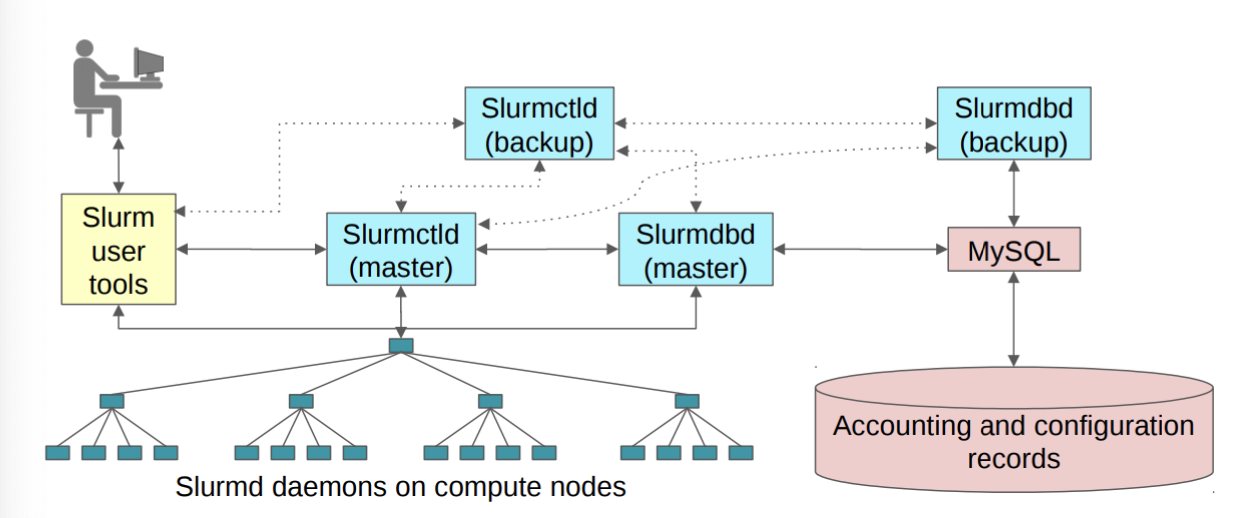
\includegraphics[width=0.8\textwidth]{assets/fig16.png}
    \caption{SLURM architecture}
    \label{fig:slurm}
\end{figure}

\begin{table}[H]
\centering
\caption{SLURM Jobfile Parameters}
\label{tab:slurm_jobfile}
\begin{tabular}{ll}
\hline
\textbf{Directive} & \textbf{Meaning} \\ \hline
\texttt{\#!/bin/bash} & Shebang directive indicating the shell to use \\
\texttt{\#SBATCH --job-name=<job\_name>} & Assigns a name to the job \\
\texttt{\#SBATCH --output=<file.out>} & Defines the output file \\
\texttt{\#SBATCH --error=<file.err>} & Defines the error file \\
\texttt{\#SBATCH --ntasks=<num\_tasks>} & Specifies total number of tasks \\
\texttt{\#SBATCH --cpus-per-task=<cpus>} & Sets desired CPUs per task \\
\texttt{\#SBATCH --mem=<memory>} & Requests memory per node or per CPU option \\
\texttt{\#SBATCH --time=<HH:MM:SS>} & Sets maximum runtime \\
\texttt{\#SBATCH --partition=<partition>} & Selects partition (queue) \\
\texttt{\#SBATCH --qos=<qos\_class>} & Specifies quality of service class \\
\hline
\end{tabular}
\end{table}


\newpage
\section{Scientific Software}

This refers to the software above the Middleware:
\begin{itemize}
    \item User's application (parallel and serial)
    \item Parallel Libraries and Tools
    \item Mathematical/Scientific Libraries
    \item I/O libraries 
    \item Compilers
\end{itemize}

Here there is not so much standardization in HPC: every machine/app has a different software stack. Every code is optimized specifically for the hardware it runs on. This creates the so called \textbf{Dependency Hell}.
\begin{definitionblock}[Dependency Hell]
    Dependency hell is a colloquial term for the frustration of some software users who have installed software packages which have dependencies on specific versions of other software packages.
\end{definitionblock}

Thus, scientific software is:
\begin{itemize}
    \item Generally available cluster-wide 
    \item Installed in /opt/cluster/software (or similar) and mounted read-only on the nodes via nfs
    \item Generally managed by modules packages 
    \item Several versions managed by some agreement
\end{itemize}




